% ════════════════════════════════════════════════════════════════════
% SECTION 4 — SYSTEM ARCHITECTURE AND METHODOLOGY
% ════════════════════════════════════════════════════════════════════
\section{System Architecture and Methodology}\label{sec:method}

\subsection{Architecture overview}

\begin{sloppypar}
Figure~\ref{fig:arch} shows the complete system. Six regional
observatory clients---stand-ins for NASA/NOAA, ESA (PROBA-2), JAXA,
ISRO, KASI, and BoM---each hold a private, non-IID shard of the
benchmark. In every communication round, each selected client trains a
local copy of the shared model on its shard (with local rebalancing and
an imbalance-robust loss, described below), and returns only its weight
increment to the aggregation server. The server forms the next global
model with distribution-aware weighted averaging, broadcasts it to all
clients, and the cycle repeats for $T = 50$ rounds. Downstream of
federation, the global model is calibrated for operations: its flare
probabilities pass through the $F_\beta$-optimal threshold and become
GIC early-warning decisions, which plug into existing SCADA workflows
for grid management. The division of labour is
deliberate: everything that touches raw magnetogram data (loading,
rebalancing, local training) executes inside the client boundary;
everything the server touches is a weight tensor.
\end{sloppypar}

\begin{figure}[t]
    \centering
    \begin{adjustbox}{max width=\textwidth, max height=0.46\textheight}
        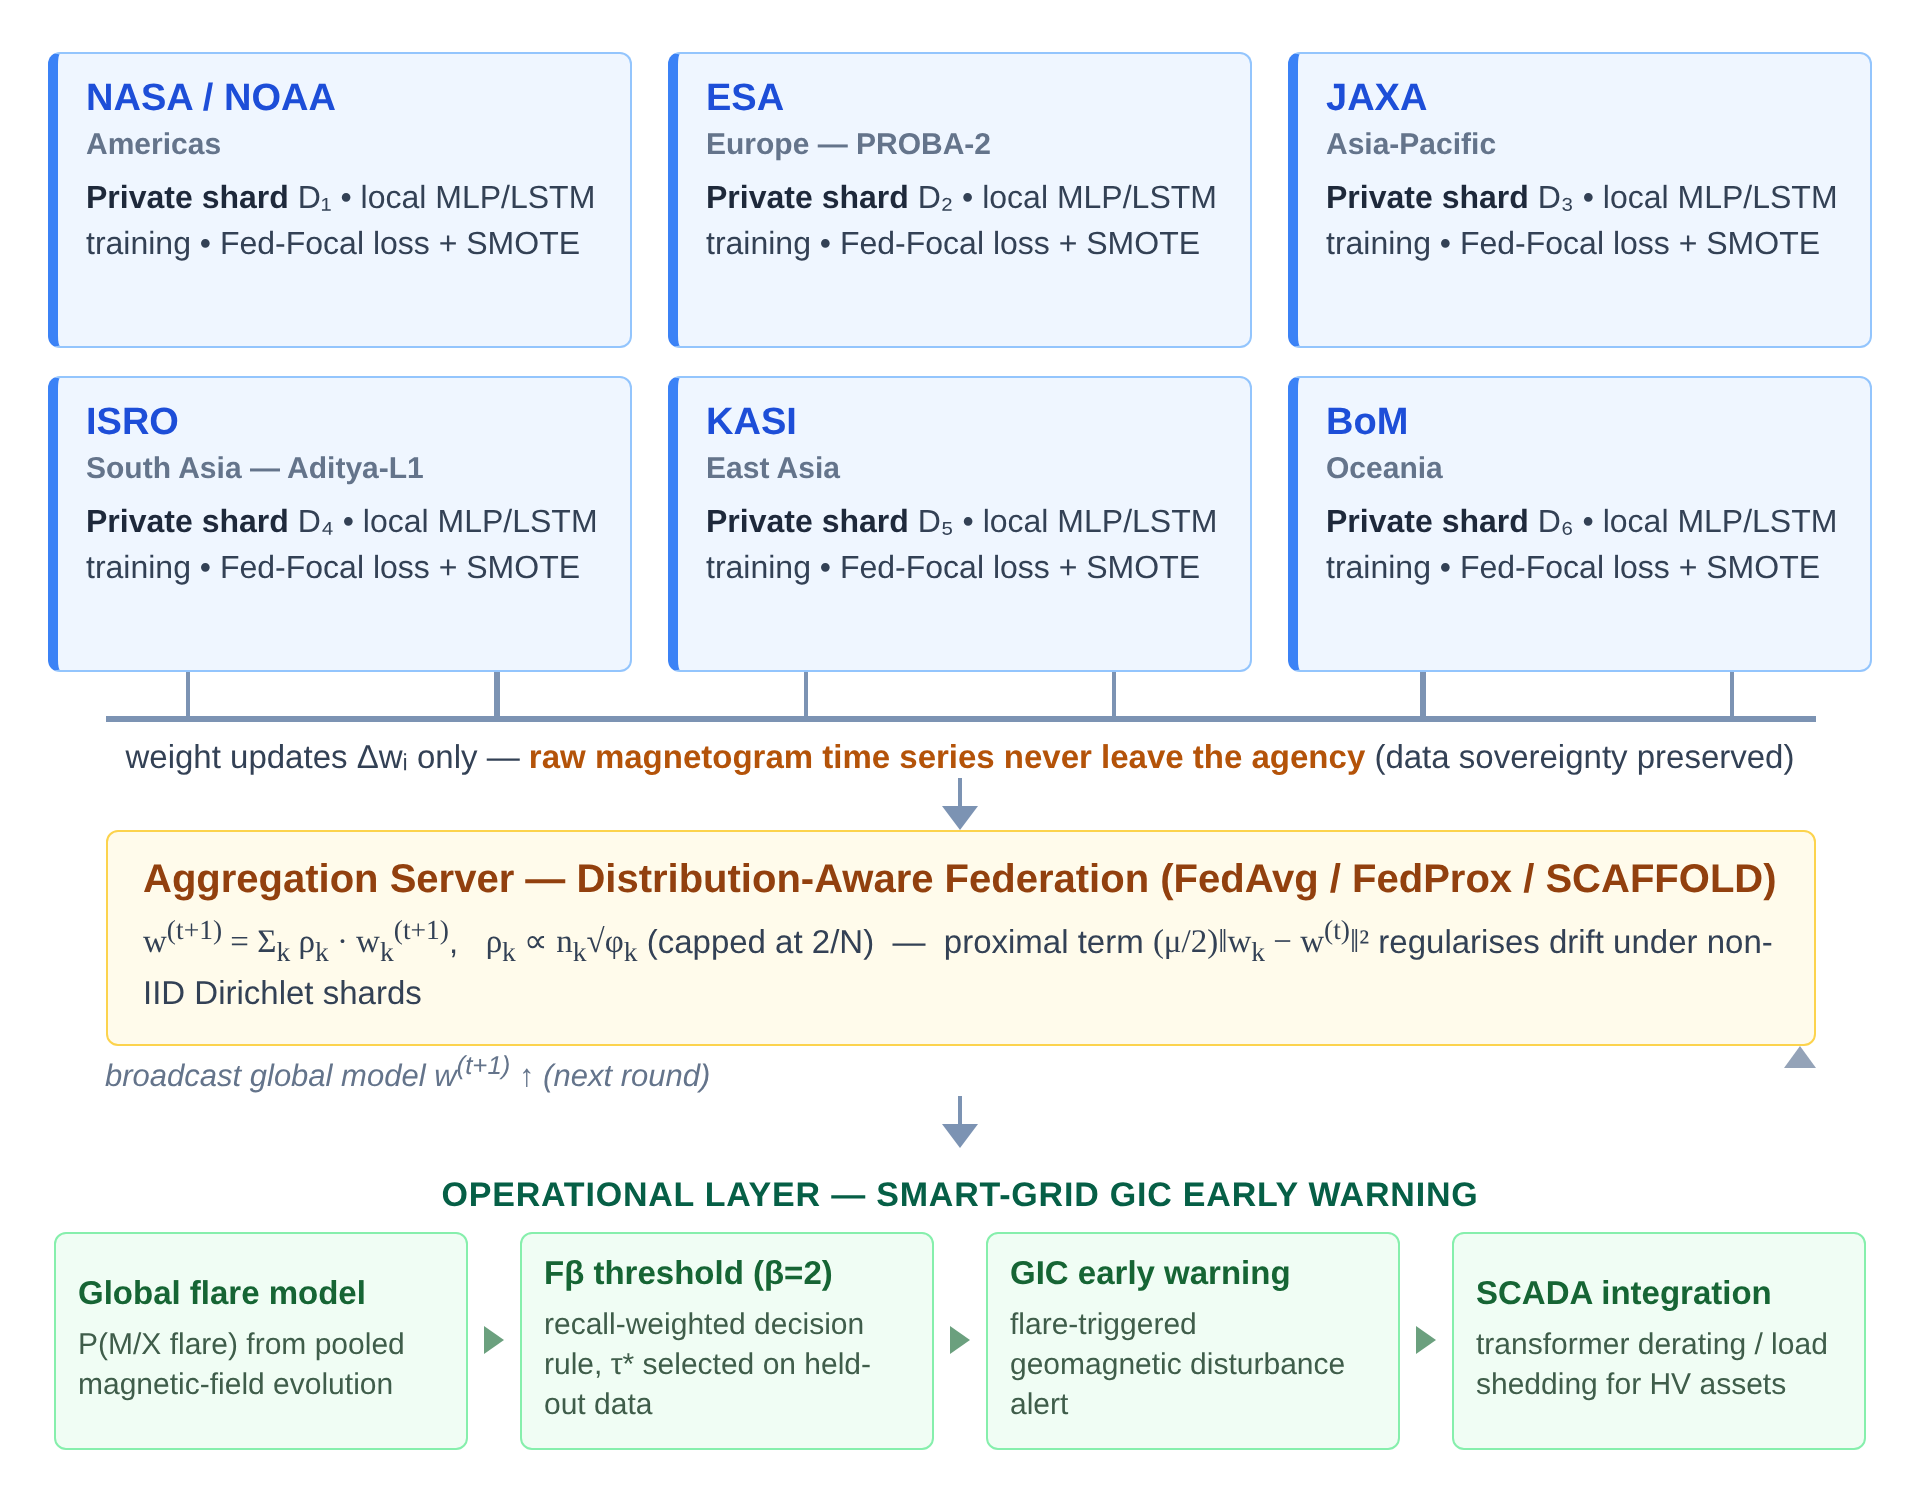
\includegraphics{figures/fig_architecture.png}
    \end{adjustbox}
    \caption{Federated space-weather monitoring architecture for
    smart-grid protection. Six regional observatory clients hold
    private non-IID shards of the benchmark; only weight updates
    $\Delta \w_k$ cross the agency boundary. The aggregation server
    applies FedAvg/FedProx with distribution-aware weighting
    ($\rho_k \propto n_k\sqrt{\phi_k}$, capped at $2/K$). The global
    model feeds an $F_\beta$-optimal decision layer for GIC early
    warning and SCADA integration.}
    \label{fig:arch}
\end{figure}

\subsection{Data: the SWAN-SF benchmark and its cleaned variant}

All experiments use the SWAN-SF benchmark \cite{angryk2020}
(doi:10.7910/DVN/EBCFKM), a multivariate time-series dataset of
active-region observation windows drawn from SDO/HMI vector
magnetograms, with 24 physically motivated parameters per timestep
sampled over 60-minute sliding windows and labels indicating the
occurrence of $\geq$M-class flares within the prediction horizon. The
24 parameters summarise magnetic-field complexity and include, among
others: total unsigned current helicity (TOTUSJH), total photospheric
magnetic free energy (TOTPOT), total unsigned vertical current
(TOTUSJZ), total unsigned flux (USFLUX), the sum of absolute
net-current-per-polarity (SAVNCPP), absolute net current helicity
(ABSNJZH), mean shear angle and the fraction of high-shear area
(MEANSHR, SHRGT45), the Schrijver flux-emergence proxy (R-value), and
the three components of the total Lorentz force (TOTFX, TOTFY, TOTFZ)
\cite{schrijver2007,bobra2015}.

We ingest the benchmark through its community-maintained cleaned
variant\footnote{Cleaned SWAN-SF Dataset,
\url{https://github.com/samresume/Cleaned-SWANSF-Dataset}, which
applies per-partition preprocessing: random undersampling with Tomek
links and TimeGAN-based synthetic augmentation for the training
partitions \cite{yoon2019}, LSBZM normalisation, and FPC-KNN
imputation.}, combining all five data partitions. The training
partitions are class-balanced by this preprocessing (pooled positive
rate $\bar{p} \approx 0.489$), while the untouched test partitions
retain the natural, severely imbalanced prevalence of approximately
$1.9\%$ flare windows across roughly $3.3\times10^{5}$ held-out
samples. This train--test contrast is not an artefact we introduce; it
is inherited from the benchmark's design philosophy, and it has a
consequence that shapes the entire evaluation: models trained at
$\sim$49\% prior must detect events at a $\sim$2\% prior, so absolute
probability calibration degrades and decision thresholds must be
re-optimised post hoc (Section~\ref{sec:thresholding}).

\subsection{Client-side feature representation}

The framework supports two representations of the same 60-timestep
observation windows. In the MLP path used for the reported run, each
three-dimensional window $X \in \R^{60\times24}$ is reduced to a
144-dimensional statistical vector
\begin{equation}\label{eq:stats}
    \tilde{x} \;=\;
    \big[\,\mu,\;\sigma,\;\max,\;\min,\;\delta,\;s\,\big]
    \;\in\; \R^{144},
\end{equation}
where each block is applied per base feature: $\mu$ and $\sigma$ are
the temporal mean and standard deviation, $\max$ and $\min$ the window
extrema, $\delta = X_{T} - X_{1}$ the net trend, and $s$ the
least-squares slope against normalised time. This six-statistic
extraction preserves substantially more temporal information than a
temporal mean (peaks, volatility, and rate of change are precisely the
flare-relevant quantities) while remaining compatible with
weight-averaged federation and with the centralised baselines. In the
LSTM path, the raw $\R^{60\times24}$ tensor is consumed directly by a
recurrent model; this path is fully implemented in the released code
but the committed artefacts analysed here correspond to the MLP
execution, and we flag the LSTM evaluation as future work
(Section~\ref{sec:limitations}).

\subsection{Non-IID partitioning into regional observatories}

\begin{figure}[t]
    \centering
    \begin{adjustbox}{max width=0.94\textwidth, max height=0.36\textheight}
        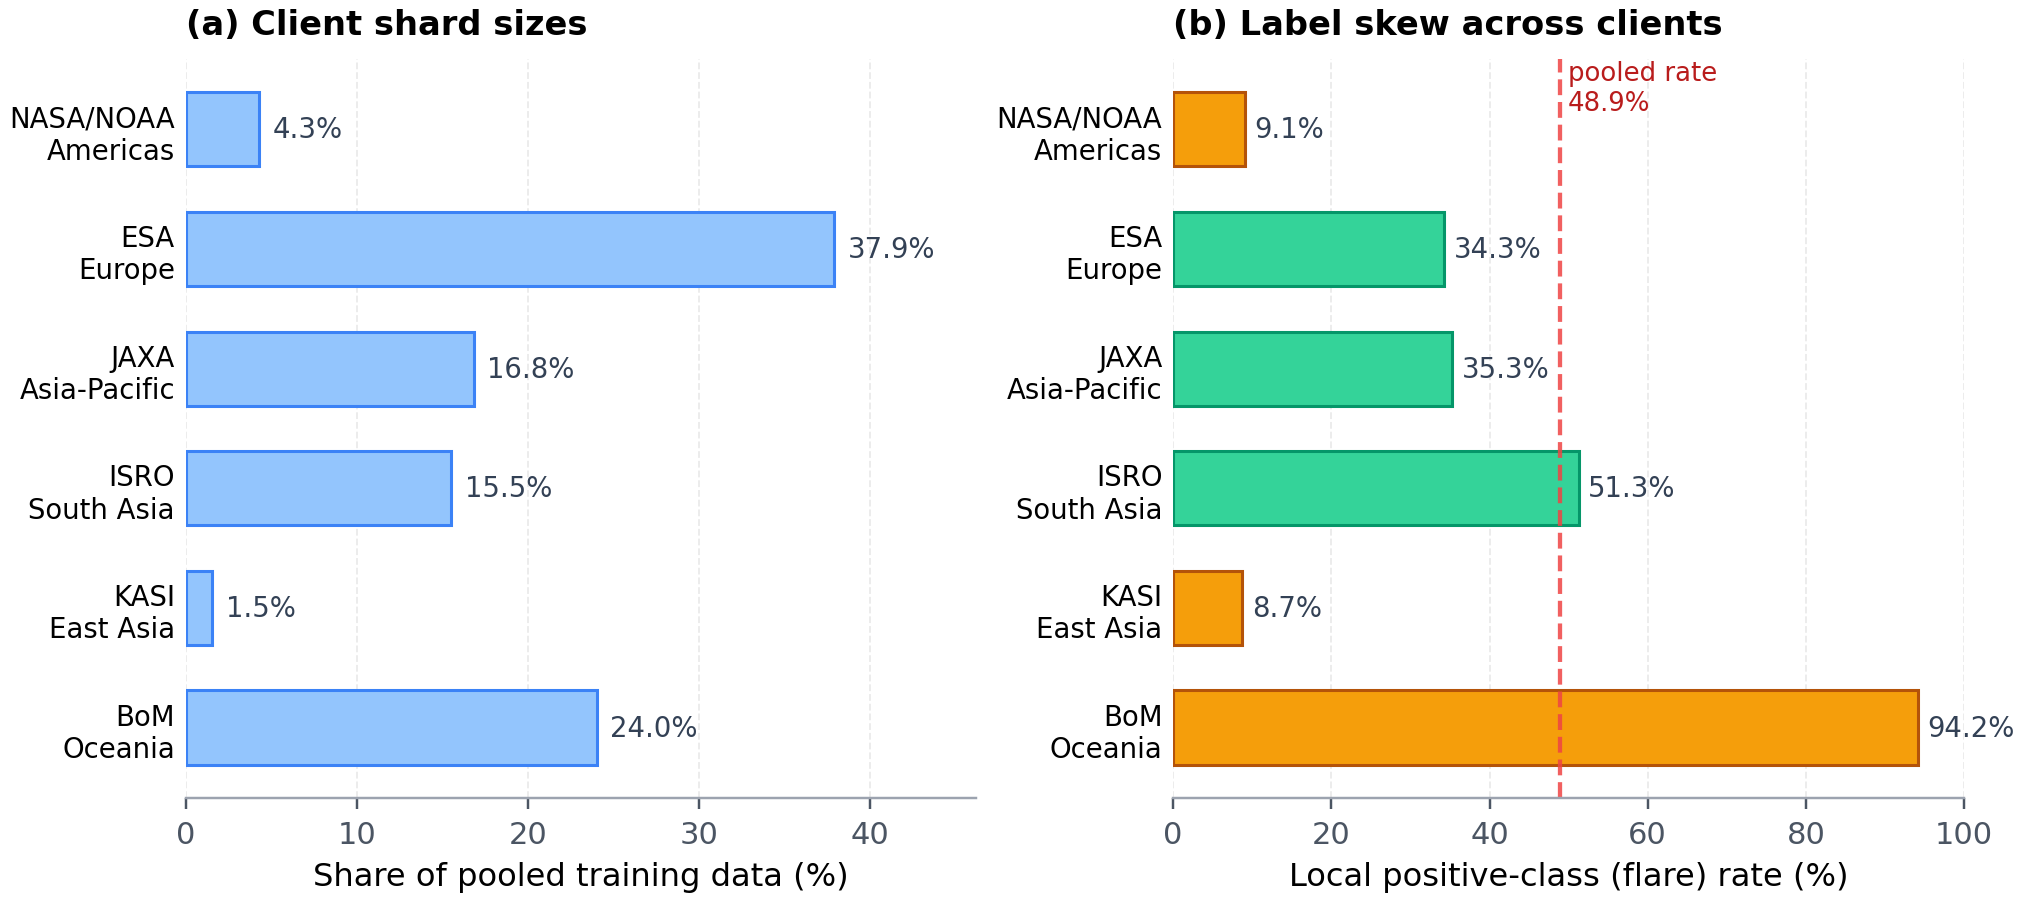
\includegraphics{figures/fig_partition.png}
    \end{adjustbox}
    \caption{Non-IID partitioning of the pooled, class-balanced
    training data into six regional clients by symmetric Dirichlet
    sampling (concentration $\alpha = 1.0$, RNG seed 42,
    Section~\ref{sec:method}). (a)~Realised relative shard sizes.
    (b)~Realised local flare rates against the pooled rate of 48.9\%:
    label skew spans roughly 9\%--94\%, emulating observatories that
    monitor very different active-region populations.}
    \label{fig:partition}
\end{figure}

To emulate geographic heterogeneity, the pooled training set is
partitioned by label-aware Dirichlet sampling: for each class $c$, a
proportion vector is drawn from
$\mathrm{Dirichlet}(\alpha,\dots,\alpha) \in \R^{K}$ and each client
receives the corresponding fraction of that class. The concentration
$\alpha$ controls heterogeneity strength---small $\alpha$ produces
near-exclusive class ownership; large $\alpha$ approaches IID.
Figure~\ref{fig:partition} shows the deterministic realisation
generated by the released configuration ($\alpha=1.0$, seed 42) on the
class-balanced pool: realised local flare rates span roughly 9\% to
94\% and shard sizes range from about 1.5\% to 38\% of the pool. This
is a deliberately hostile federation: some clients are flare-rich and
tiny, others flare-poor and large, mirroring the real asymmetry between
agencies whose instruments and coverage dominate the corpus and those
monitoring smaller regional populations. The concentration $\alpha=1.0$
itself is the outcome of a documented tuning process
(Appendix~\ref{sec:appendix}): early experiments at $\alpha \le 0.5$
produced pathological partitions (0.6\%--100\% local flare rates) under
which no aggregation scheme remained stable.

\subsection{Client models}

The primary federated architecture is a four-layer multilayer
perceptron, $\mathrm{SolarMLP}: \R^{144} \to \R$, with hidden widths
$144 \to 128 \to 64 \to 32 \to 1$, batch normalisation, ReLU
activations, and dropout $0.3$ after each hidden layer; the single
output is a raw logit consumed by the sigmoid-based losses below. MLPs
are natural federation citizens because every parameter is a
numerically meaningful averageable tensor. The released framework also
implements $\mathrm{SolarLSTM}$, a (optionally bidirectional) two-layer
LSTM with hidden size 128, Xavier/orthogonal initialisation, and a
forget-gate bias of one for long-horizon memory, followed by a
two-layer classification head \cite{hochreiter1997,hassani2025}. Local
training uses AdamW \cite{loshchilov2019} with cosine-annealing warm
restarts and gradient-norm clipping at $5.0$. We deliberately keep
XGBoost out of the federation loop: gradient-boosted tree ensembles
store discrete structure that cannot be meaningfully averaged, so the
centralised XGBoost serves as the pooled upper bound rather than a
federated participant.

\subsection{Federation algorithms and aggregation}

Three cross-silo algorithms are implemented. \textbf{FedAvg}
\cite{mcmahan2017}: each round, every client initialises from the
broadcast global model, performs $E=10$ local epochs, and the server
averages the returned weights. \textbf{FedProx} \cite{li2020}: identical
to FedAvg except each client's local objective is regularised by the
proximal term of Eq.~\eqref{eq:fedprox} with
$\mu = 0.01$, penalising drift from the global model---the mechanism
we hypothesise is decisive under the label skew of
Figure~\ref{fig:partition}. \textbf{SCAFFOLD} \cite{karimireddy2020}:
variance reduction via client and server control variates; it is
implemented with the SGD-based update required for exactness of the
control-variate correction, but is disabled in the released
configuration pending stability work, and we exclude it from the
reported comparison (Section~\ref{sec:appendix}).

Aggregation is \emph{distribution-aware} in both FedAvg and FedProx
runs: the server weights client $k$'s update by
\begin{equation}\label{eq:dafl}
    \rho_k \;\propto\; n_k \sqrt{\phi_k},
    \qquad
    \phi_k = \frac{p_k}{\bar{p}},
    \qquad
    \rho_k \le \frac{2}{K},
\end{equation}
where $p_k$ is the client's local positive rate and $\bar{p}$ the
pooled rate known to the server. The square-root damping and the
$2/K$ cap prevent a flare-rich client from dominating the global
model while still up-weighting the clients most likely to contain
decision-relevant minority samples. Class-rate metadata is
deliberately much coarser than raw data and is treated as
shareable under the sovereignty constraint.

\subsection{Fed-Focal loss and local rebalancing}

Each client rebalances its shard locally with SMOTE
\cite{chawla2002} to a minority fraction of $0.25$ and trains with a
server-aware focal loss in the Fed-Focal family \cite{sarkar2020},
\begin{equation}\label{eq:focal}
    \ell_{\mathrm{fedfocal}}
    \;=\; -\,\alpha_t\,\bigl(1 - p_t\bigr)^{\gamma}
    \log\bigl(p_t\bigr),
    \qquad \gamma = 2.0,
\end{equation}
where $p_t$ is the model's probability of the correct class and
$\alpha_t$ interpolates between $\alpha$ and $1-\alpha$ by label. The
positive-class weight $\alpha$ is computed per client as the base value
$0.25$ \cite{lin2017} scaled by a square-root-damped imbalance factor
$\min\!\big(\sqrt{\bar{p}/p_k},\,1.5\big)$ and a mild round-progress
factor, then clamped to $(0.05, 0.25)$. This clamping is a hard-won
design decision: unclamped adaptive weighting (earlier versions allowed
$\alpha$ up to $0.95$) systematically inflated positive-class weight on
flare-poor clients, producing degenerate always-flare classifiers with
recall $\approx 1.0$ and precision $\approx 0.03$
(Appendix~\ref{sec:appendix}). NaN-safe clamping of $p_t$ and of the
loss itself guards the pipeline against logit explosions in early
rounds.

\subsection{Threshold optimisation for safety-critical recall}
\label{sec:thresholding}

Because federated training operates on rebalanced local data while
deployment operates at the natural $1.9\%$ prior, the emitted
probabilities are deliberately miscalibrated, and a fixed $0.5$
threshold is meaningless. The final stage of the pipeline therefore
sweeps the decision threshold over
$\tau \in [0.10, 0.90]$ in steps of $0.01$ and selects, per model, the
$\tau^\ast$ that maximises $\Fbeta$ with $\beta=2$
(Eq.~\eqref{eq:fbeta}) on the held-out test set. All reported
precision, recall, F1, and accuracy figures are taken at each model's
$\Fbeta$-optimal threshold; ROC-AUC, being threshold-free, is reported
independently. We follow the pipeline's evaluation code in treating
threshold selection as part of the operational calibration rather than
as test-set leakage; Section~\ref{sec:limitations} discusses the
stricter alternative of selecting $\tau^\ast$ on a validation split.

\subsection{Interpretability layer}

To audit what the models learn, SHAP values \cite{lundberg2017} are
computed for the centralised XGBoost surrogate over a 500-sample test
subset with the TreeExplainer, yielding mean absolute SHAP
attributions per feature. Because the statistical representation of
Eq.~\eqref{eq:stats} names features generically
(\texttt{feature\_0}, \dots, \texttt{feature\_143}) in the released
pipeline, we decode the indices analytically: the concatenation order
is $\mu$ (0--23), $\sigma$ (24--47), $\max$ (48--71), $\min$
(72--95), $\delta$ (96--119), $s$ (120--143), each block ordered by the
24 base parameters. Section~\ref{sec:results} presents both the raw
ranking and its decoded physical reading.
